\section{自定义章节标题一}
\subsection{第一章第1节}\qanswerloc{10}

\begin{questions}[r]

    \begin{bbox}
        \question   设$f(x)$满足$2f(x)+f(1-x)=x^2$,则$f(x)=\blankline.$
    \end{bbox}

    \begin{bbox}
        \question   设$f(x)=2x+\sqrt{x^{2}+2x+1}$,$g(x)=
        \begin{cases}
        x+2, & x\geqslant0, \\
        x-1, & x<0,  
        \end{cases}$,则$g[f(x)]= \blankline$.
    \end{bbox}

    \begin{bbox}
        \question   设某项目用于 发和宣传 总成本为$a$万元 当 发和宣传所 成本分别为$x$万元和 $y$ 万元时, 收益为$R=2x^{\frac{1}{3}}y^{\frac{1}{2}}$万元,则收 最大时,研发所用成本为\blankline.
    \end{bbox}

    \begin{bbox}
        \question   已知 $\lim\limits_{x\to0}\dfrac{f(x)}{x}$ 存在,且函数
        $$f(x)=\ln(1+x)+2x\bullet\lim_{x\to0}\frac{f(x)}{\sin x}$$
        则$\lim\limits_{x\to0}\dfrac{f(x)}{x}=$ \blankline.
    \end{bbox}

    \begin{bbox}
        \question  可以用\blankbox 定义一个完整的数据结构。\textwater

        \fourchoices{数据元素}{数据对象}{数据关系}{抽象数据类型}     
    \end{bbox}

    \begin{bbox}
        \question   若某算法的空间复杂度为$O(1)$,则表示该算法\blankbox 。
        \fourchoices
        {不需要任何辅助空间}
        {所需辅助空间大小与问题规模$n$无关}
        {不需要任何空间}
        {所需空间大小与问题规模$n$无关}
    \end{bbox}
\end{questions}

\subsection{第一章第2节}
\qanswerloc{15}

\begin{questions}[tr]

    \begin{bbox}
        \question   下列关于时间复杂度的函数中,时间复杂度最小的是\blankbox 。
        \fourchoices
        {$T_1(n)=n\log_2n +5000n$}
        {$T_2(n)=n^2 - 800n$}
        {$T_3(n)=n\log_2n - 6000n$}
        {$T_4(n)=20000\log_2n$}
    \end{bbox}

    \begin{bbox}
        \question   【2017 统考真题】 下列函数的时间复杂度是 \blankbox 。
        \begin{lstlisting}
    int func(int n){
        int i=0, sum=0;
        while(sum<n) sum += ++i;
        return i;
    }
        \end{lstlisting}
        \fourchoices{$O(\log n)$}{$O(n^{\frac{1}{2}})$}{$O(n)$}{$O(n\log n)$}
    \end{bbox}

\end{questions}

\section{自定义章节标题二}
\subsection{第二章第1节}
\qanswerloc{20}
\begin{questions}[tr]
    
    \begin{bbox}
        \question  已知曲线$L:y=\ln\sqrt{x}(2\leqslant x\leqslant4)$,在$L$ 上的任意点$P(x,y)$作切线,记切线与曲线$L$在 $2\leqslant x\leqslant4$
        时所围成的有界区域的面积为$S$.
        \begin{subquestions}
            \subquestion 求一点$P_0$,使上述面积$S$关于$x$的变化率为零;
            \subquestion 当点$P(x,y)$在曲线上移动至$(\mathrm{e},\dfrac{1}{2})$时,横坐标关于时间的变化率为1,求此时面积关于时间的变化率$\dfrac{\mathrm{d}S}{\mathrm{d}t}.$
        \end{subquestions}

    \end{bbox}

    \begin{bbox}
        \question 以 $yOz$ 面上的平面曲线段$y=f(z)(z\geqslant0)$ 绕$z$轴旋转一周所成旋转曲面与xOy 面围成一个无上盖容器(见图),现以 3 cm$^3/$s 的速率把水注人容器内,水面的面积以$\pi$ c$m^2$/ s 的速率增大.已知容器底面积为 16$\pi$ c$m^2$,求曲线$y=f(z)$的方程.
        \imgin{0.2}{fig/img01.png}

        % 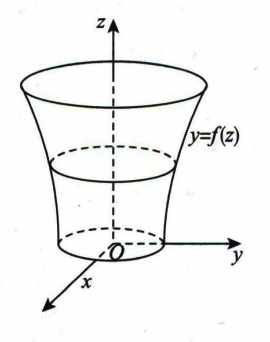
\includegraphics[width=0.2\textwidth]{img/img01.png}
    \end{bbox}

    \begin{bbox}
        \question   分析以下各程序段, 求出算法的时间复杂度.
        \begin{lstlisting}[escapeinside={(*@}{@*)}]
    (*@\ding{172}:@*)
    i=1; k=0;
    while(i<n-1){
        k=k+10*i;
        i++;
    }

    (*@\ding{173}:@*)
    y=0;
    while((y+1)*(y+1)<=n)
    y=y+1;

    (*@\ding{174}:@*)
    for(i=0;i<n;i++)
        for(j=0;j<m;j++)
            a[i][j]=0;
    
        
        \end{lstlisting}
    \end{bbox}

    \begin{bbox}
        \question   【2011 统考真题】一个长度为 $L$($L\geqslant 1$ )的升序序列$ S$, 处在第$\lceil L/2\rceil $个位置的数称为 $S$
        的中位数。例如,若序列 $S_1$=(11,13,15,17,19), 则 $S_1$的中位数是 15, 两 个序列的中位
        数是含它们所有元素的升序序列的中位数。例如,若 $S_2$ =(2,4,6,8,20), 则$S_1$和$S_2$的中
        位数是 11。现在有两 个等长升序序列$A$和$B$, 试设计一个在时间和空间两 方面都尽可能
        高效的算法,找出两个序列 $A$和$B$的中位数。要求:
        \begin{subquestions}
            \subquestion 给出算法的基本设计思想
            \subquestion  根据设计思想,采用 C 或 C++或 Java 语言描述算法,关键之处给出注释
            \subquestion 说明你所设计算法的时间复杂度和空间复杂度
        \end{subquestions}
    \end{bbox}
\end{questions}